\section{System Design}
\label{sec:design}
AgentWorkShop is designed for industrial tasks whose agents, production
contexts, interfaces, and process signals vary between deployments. A useful
framework must let these differences be configured without changing the
shared task runtime, while ensuring that a proposed operation is checked
against the active production context before it reaches a device. It must also
retain enough route-specific evidence to distinguish a returned command
receipt from a measured process response.

\subsection{Design Rationale and Requirements}
\label{sec:principles}
The five requirements---scene variability, harness variability, operation
authority, observability, and extensibility---organize six design rules
(D1--D6). They are deployment constraints selected from the target workflows,
not a taxonomy inferred from a systematic review or an empirical coding study:
encode scene settings as versioned data; extend the runtime through registered
harness, tool, and driver interfaces; separate proposal from execution; treat
the tool catalog as discovery rather than permission; route actuator writes
through the common DCW admission point; and retain evidence by operation.
D1 maps to blueprints and context resolution; D2 to the harness, tool, and
driver registries; D3--D5 to task dispatch, binding/grant checks, and DCW
write admission; and D6 to route handlers and the evidence ledger. The
evaluation maps these rules to complementary evidence: Q1 and Q4 exercise
historical direct-node scene mappings; Q2 exercises two tasks with one
registered OMP harness; Q5 checks dispatcher and write-confirmation regressions
on v0.7.57; Q6 and the October 23 boundary record exercise recipe and approval
paths; and Q7 checks current v0.8.0 protocol acquisition, bounded writes,
readback, and data lineage across two simulator scenes. Q7 does not traverse
the registered harness or demonstrate profile adaptation, and these evidence
units do not form one end-to-end deployment trial. The results state available
version and interface provenance and identify gaps, including the unavailable
R1 runtime worktree and R6 commit. AgentWorkShop does not select an agent's
control strategy or replace independent controller and safety functions.

\subsection{Layered Architecture}
\label{sec:layers}
\label{sec:arch}
Fig.~\ref{fig:arch} maps the reference implementation onto six bands and a
shared evidence ledger. The access band exposes command-line, web, SDK, REST,
MCP, and A2A entry surfaces. The collaboration band contains workspaces,
channels, task queues, shared memory, mailboxes, task templates, and
harness adapters. The governance band projects an operation catalog and
checks each invocation. The context band binds a scene blueprint to the
active line--product--recipe--run tuple and its semantic DAQ/DCW nodes. The
service band provides acquisition, write control, analysis, retrieval, and
optional model services. The field-I/O band resolves semantic nodes to
built-in or plugin drivers for a plant or simulator.

Each band has a distinct responsibility. Entry surfaces converge on the
same task runtime; a harness adapter supplies the agent-specific interaction;
semantic nodes hide protocol details from the task; and the driver registry
provides the device-facing extension point. The evidence ledger records
task, command, observation, and version events against their actor and
production context. It does not collapse them into a single success flag.

\subsection{Cross-Module Execution Flow}
\label{sec:executionflow}
Fig.~\ref{fig:runtime} summarizes a task turn from entry to returned
evidence. The runtime resolves the production context and assembles the
prompt and scoped tool catalog before invoking a registered harness. For
each returned tool call, the shared dispatcher rechecks invocation scope
and channel policy; industrial operations also receive current grant and
binding checks before handler selection. The selected handler applies its
own route-specific guards, approval, revalidation, and device-I/O steps.
Command receipts and any later process observations remain distinct records.

Fig.~\ref{fig:execution} gives pseudocode for these cross-module contracts;
it is a reference flow rather than one literal orchestrator function.
Route-specific timing, approval, and evidence rules are detailed in
Section~\ref{sec:modules}.

\begin{figure*}[!t]
\centering
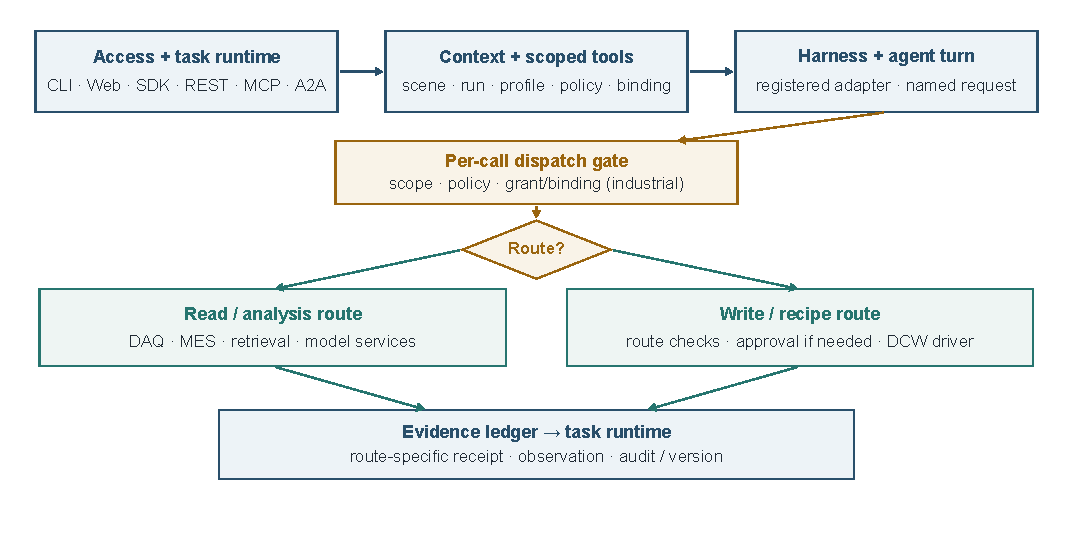
\includegraphics[width=\textwidth]{resources/fig-runtime-2026.pdf}
\caption{Cross-module task execution in AgentWorkShop. Entry and task
services assemble the channel-scoped tool catalog before the agent turn;
each returned call is rechecked for scope and policy, with grant and binding
checks for industrial operations. Dispatch-gate refusals stop before handler
execution, whereas route-specific handlers may read state before refusing a
write. Receipts and later observations remain distinct.}
\label{fig:runtime}
\end{figure*}

\begin{figure}[!t]
\centering
\begin{algorithmic}[1]
\Require task $q$, channel $c$, bound agent $a$
\Ensure task result and route-linked evidence
\State $x \gets \Call{ResolveContext}{c,q}$
\State $T \gets \Call{FilterToolCatalog}{a,c}$
\State $m \gets \Call{RetrieveMemory}{q}$
\State $p \gets \Call{AssemblePrompt}{q,x,m}$
\State $h \gets \Call{InvokeRegisteredHarness}{a,p,T}$
\ForAll{tool request $u$ returned by $h$}
  \State $g \gets \Call{CheckScopeAndChannelPolicy}{a,c,u}$
  \If{\textbf{not} $g$}
    \State \Call{RecordDispatchRefusal}{u,x}; \textbf{continue}
  \EndIf
  \If{$u$ is an industrial operation}
    \State $v \gets \Call{CheckGrantAndBinding}{a,u}$
    \If{\textbf{not} $v$}
      \State \Call{RecordDispatchRefusal}{u,x}; \textbf{continue}
    \EndIf
  \EndIf
  \State $k \gets \Call{SelectHandler}{u}$
  \State $r \gets \Call{ExecuteRouteHandler}{k,u,x}$
  \State \Call{RecordAvailableEvidence}{u,r,x}
  \State \Call{ReturnToolResult}{h,r}
\EndFor
\State \Return task state and retained evidence
\end{algorithmic}
\caption{Reference pseudocode for cross-module execution in AgentWorkShop.}
\label{fig:execution}
\end{figure}
